% Created 2020-09-09 mié 10:19
% Intended LaTeX compiler: pdflatex
\documentclass[11pt]{article}
\usepackage[utf8]{inputenc}
\usepackage[T1]{fontenc}
\usepackage{graphicx}
\usepackage{grffile}
\usepackage{longtable}
\usepackage{wrapfig}
\usepackage{rotating}
\usepackage[normalem]{ulem}
\usepackage{amsmath}
\usepackage{textcomp}
\usepackage{amssymb}
\usepackage{capt-of}
\usepackage{hyperref}
\hypersetup{colorlinks=true,urlcolor=blue}
\usepackage{fancyhdr}
\fancyhead{} % clear all header fields
\pagestyle{fancy}
\fancyhead[R]{1-SMX}
\fancyhead[L]{Unidad 01: Sistemas Operativos]}
\usepackage{wallpaper}
\ULCornerWallPaper{0.9}{../rsrc/logos/header_europa.png}
\CenterWallPaper{0.7}{../rsrc/logos/watermark_1.png}
\author{Angel Berlanas Vicente}
\date{\today}
\title{Unidad 01 - Introducción y Virtualización}
\hypersetup{
 pdfauthor={Angel Berlanas Vicente},
 pdftitle={Unidad 01 - Introducción y Virtualización},
 pdfkeywords={},
 pdfsubject={},
 pdfcreator={Emacs 26.3 (Org mode 9.1.9)}, 
 pdflang={English}}
\begin{document}

\maketitle
\tableofcontents

\newpage
\section{Introducción a los Sistemas Operativos}
\label{sec:org23c28fc}

\subsection{Introducción}
\label{sec:orga4aa5ae}

En este primer tema nos centraremos conocer bien ¿Qué es un \emph{Sistema Operativo}?, 
así como las funciones que tiene.

Veremos que existen multitud de Sistemas Operativos, cada uno adaptado al propósito
que deben cumplir.

\subsection{¿Qué es un Sistema Operativo?}
\label{sec:org27f6240}
Desde el punto de vista del usuario, el sistema operativo consiste en
una serie de programas y funciones que ocultan los detalles del
hardware,ofreciéndole una vía sencilla y flexible de acceso al mismo,
teniendo dos objetivos fundamentales:

\subsubsection{Seguridad}
\label{sec:orgf7b7045}
El sistema operativo debe actuar contra cualquier manipulación extraña,
ya sea accidental o premeditada que pudiera dañar la información,
perjudicar a otros usuarios o provocar un funcionamiento indeseado del
sistema. Por ejemplo, hay ciertas instrucciones que pueden parar la
máquina y otras que realizan operaciones directamente sobre el hardware,
que debemos evitar que se utilicen por los programas. Para ello, algunos
sistemas proporcionan dos estados, llamados estado protegido (Sistema o
\texttt{Kernel}), en el cual se ejecuta el sistema operativo, y estado no
protegido (Usuario o User), que es el destinado a la ejecución de los
programas de usuario y de aplicación. De esta manera se impide que los
programas de los usuarios puedan tener contacto directo con el hardware,
o puedan forzar un incorrecto funcionamiento del sistema.

\begin{center}
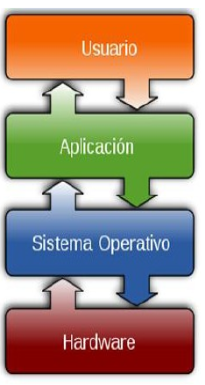
\includegraphics[width=5cm]{ArquitecturaSistemaOperativo/SO_Capas.PNG}
\end{center}

\subsubsection{Abstracción}
\label{sec:org84b7b74}
La tendencia actual del software y de los lenguajes de programación, que iremos viendo 
en otros cursos, es ocultar lo más posible los detalles de más bajo nivel, intentando dar a
los niveles superiores una visión más sencilla, global y abstracta, ofreciéndoles operaciones 
para manipular dichas estructuras ocultas, desconociendo por completo la gestión interna de las mismas. 

Sobre estas estructuras se construyen otras que abstraen a las anteriores, y así
sucesivamente. 

Gracias a la abstracción, los sistemas operativos enmascaran los recursos físicos, permitiendo su manejo con funciones más
generales que ocultan las básicas, constituyendo verdaderos recursos ficticios o virtuales, que mejoran y son más potentes que los físicos.

Desde el punto de vista de un programa o usuario, la máquina física se convierte, en una máquina extendida, que presenta la ventaja respecto a
la física de ofrecer más funciones de las que normalmente soportaría esta última. 

Entre las posibilidades de esto estarían:

\begin{itemize}
\item Las carpetas compartidas.
\item Los usuarios en red.
\item Las impresoras compartidas.
\item Acceso a recursos ajenos al propio \emph{hardware}.
\end{itemize}

\begin{center}
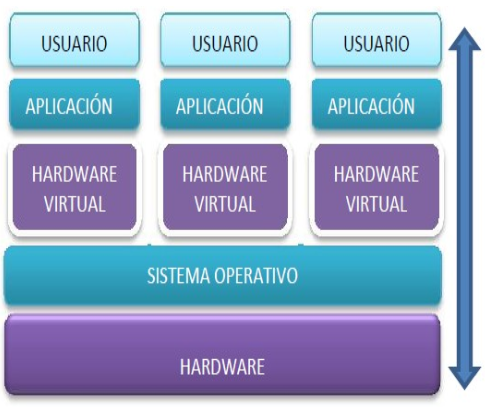
\includegraphics[width=.9\linewidth]{ArquitecturaSistemaOperativo/SO_MaquinaExtendida.PNG}
\end{center}

A modo de resumen, podemos decir que el sistema operativo persigue alcanzar
la mayor eficiencia posible del hardware y facilitar el uso del mismo a
los usuarios y a las aplicaciones.

\subsection{Aviso a Navegantes}
\label{sec:org0c68f1e}

Lo descrito anteriormente da lugar a una situación para la mayor parte de los usuarios, que es la creencia de que 
\emph{todo es mágia}.

\begin{figure}[htbp]
\centering

\includegraphics[width=10cm]{./ArquitecturaSistemaOperativo/mago.jpg}
\caption{"Los ficheros los crea un mago"}
\end{figure}

Como futuros Administradores de Sistemas debemos conseguir comprender el funcionamiento de dichos
procesos, abstrayéndonos lo necesario en los primeros momentos, pero profundizando cada vez más 
para comprender que es \texttt{exactamente} lo que ocurre cuando se producen eventos como :

\begin{itemize}
\item clicks de ratón.
\item enviar a imprimir.
\item crear carpetas.
\item formatear discos.
\end{itemize}

No seremos buenos profesionales si no tenemos conocimientos acerca de lo que esas acciones desencadenan 
y cómo se realizan por parte del Sistema Operativo. 

\textbf{¿Por qué esto es tan importante?}

Porque muchas veces (\emph{más de las que nos gustaría}), esos procesos fallarán y nos devolveran (\emph{o nó :-)})
mensajes de error que nos permitirán averiguar \emph{qué} está pasando y poco a poco aprenderemos \emph{cómo} arreglarlos.

A lo largo del curso nos veremos en más de una situación de estas características. No os preocupéis si no 
sabéis como arreglar el problema (\emph{para eso estais aquí}). Lo que se valorará es vuestra capacidad de analizarlo
y plantear posibles soluciones, no la solución en si misma.

\newpage
\subsection{Tarea 01 : Introducción}
\label{sec:orgc4c56fd}

Busca en Internet información acerca de los ficheros de texto plano.
Utilizando \texttt{nano}, redacta un fichero que conteste a las siguientes preguntas:

\begin{itemize}
\item ¿Qué significa \emph{abstracción} si estamos hablando de Sistemas Operativos?
\item ¿Qué es el \emph{kernel} de un Sistema Operativo?.
\item ¿Qué Sistemas Operativos has utilizado?
\end{itemize}


\newpage
\section{Funciones de los Sistemas Operativos}
\label{sec:org0538480}
Las funciones de los sistemas operativos son diversas y han ido
evolucionando de acuerdo con los progresos que la técnica y la
informática han experimentado. Como principales funciones, podríamos
enumerar las siguientes:

\subsubsection{Gestión de procesos}
\label{sec:org3ea397c}
Hay que diferenciar entre los conceptos programa y proceso. Un programa
es un ente pasivo, que cuando se carga en memoria y comienza a
ejecutarse, origina uno o varios procesos. Un \textbf{proceso} podríamos definirlo, como
\emph{parte de un programa en ejecución}.

A lo largo de las unidades que vendrán, haremos muchos ejercicios para la gestión
de los procesos.

\subsubsection{Gestión de la memoria}
\label{sec:orgee70906}
La gestión de memoria, suele ir asociada a la gestión de procesos. Para
ejecutar un proceso es necesario asignarle unas direcciones de memoria
exclusivas para él y cargarlo en ellas, cuando el proceso finalice su
ejecución es necesario liberar las direcciones de memoria que estaba
usando.

\begin{center}

\includegraphics[width=.9\linewidth]{./imgs/meme-chrome-ram.jpg}
\end{center}

\subsubsection{Gestión de ficheros}
\label{sec:orge85ac2f}
Un fichero es una abstracción para definir una colección de información
no volátil. Su objetivo es proporcionar un modelo de trabajo sencillo
con la información almacenada en los dispositivos de almacenamiento.

Estos ficheros deben tener espacio asignado en los dispositivos, deben
estar protegidos entre ellos, deben organizarse según unos determinados
esquemas\ldots{} todo esto es la gestión de ficheros.

Parece mucho más difícil de lo que és en realidad. Sin embargo el diablo está en los detalles.

Una de las máximas que aparecerán a lo largo de todo el curso es:

\emph{Todo en GNU/LinuX es un fichero}. 

O sea, que todo lo que se gestiona por parte de los Sistemas Operativos, incluido él mismo, son ficheros.

Si aprendemos a manejarnos con los ficheros, aprenderemos a gestionar los Sistemas Operativos y por tanto
los Ordenadores.

\subsubsection{Gestión de los dispositivos de E/S}
\label{sec:org26392a3}
La gestión de la entrada-salida (\emph{aka} \emph{E/S}) tiene como objetivo proporcionar
una interfaz de alto nivel de los dispositivos de E/S sencilla de
utilizar, tanto por parte de propio Sistema Operativo y los procesos que 
se ejecutan en él, como por parte del usuario.

Veremos en este punto conceptos como:

\begin{itemize}
\item Drivers (\emph{controladores}).
\item Discos.
\item Impresoras.
\item Monitores.
\item Teclado y Ratón.
\end{itemize}

\subsubsection{Gestión de la red}
\label{sec:org8463cb0}
El sistema operativo es el encargado de gestionar los distintos niveles
de red, los drivers (controladores) de los dispositivos involucrados en
la red, los protocolos de comunicación, las aplicaciones de red, etc.

Muchas de las prácticas que haremos a lo largo del curso tienen que ver con este apartado,
ya que en el mundo en el que vivimos, casi cualquier dispositivo \emph{necesita} de una 
conexión a Internet (o al menos a una red local (\emph{LAN})).

\subsubsection{Protección y seguridad}
\label{sec:org6c35055}
Mecanismos para permitir o denegar el acceso a los usuarios y a sus
procesos a determinados recursos (ficheros, dispositivos de E/S, red,
etc.).

\newpage

\section{Tipos de Sistemas Operativos}
\label{sec:org3bd1d4d}
Existen muchas categorizaciones, pero una de las más comunes es la de
los servicios que ofrece.

\begin{center}
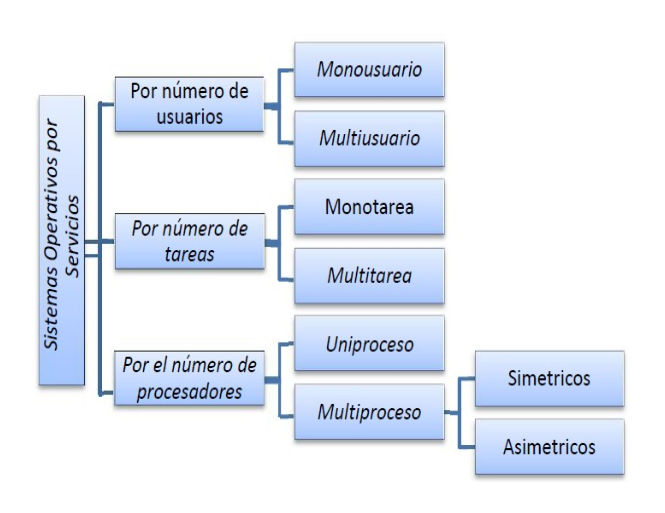
\includegraphics[width=.9\linewidth]{ArquitecturaSistemaOperativo/SO_Tipos.PNG}
\end{center}

\subsubsection{Según el número de usuarios}
\label{sec:orga53f1ad}
\begin{enumerate}
\item Monousuarios
\label{sec:org0bc4906}
Los sistemas operativos monousuarios son aquéllos que soportan a un
usuario a la vez, sin importar el número de procesadores que tenga la
computadora o el número de procesos o tareas que el usuario pueda
ejecutar en un mismo instante de tiempo.

Sistemas Operativos Monousuario:

\begin{itemize}
\item MS-DOS
\item Windows 95
\item Windows 98
\end{itemize}

\item Multiusuario
\label{sec:org1bdda3e}
Los sistemas operativos multiusuario son capaces de dar servicio a más
de un usuario a la vez, ya sea por medio de varias terminales conectadas
a la computadora o por medio de sesiones remotas en una red de
comunicaciones. No importa el número de procesadores en la máquina ni el
número de procesos que cada usuario puede ejecutar simultáneamente.

Sistemas Operativos Multiusuario:

\begin{itemize}
\item UNIX-GNU/LinuX
\item Windows NT (en adelante)
\end{itemize}
\end{enumerate}


\subsubsection{Sistemas Operativos Distribuidos}
\label{sec:org8699c0c}
Un sistema distribuido se define como una colección de equipos
informáticos separados físicamente y conectados entre sí por una red de
comunicaciones distribuida; cada máquina posee sus componentes de
hardware y software de modo que el usuario percibe que existe un solo
sistema (no necesita saber qué cosas están en qué máquinas). El usuario
accede a los recursos remotos de la misma manera en que accede a
recursos locales ya que no percibe que existan varios ordenadores, sino
que solo es capaz de ver uno formado por todos los anteriores. Una
ventaja fundamental de los sistemas distribuidos, es que permiten
aumentar la potencia del sistema informático, de modo que 100
ordenadores trabajando en conjunto, permiten formar un único ordenador
que sería 100 veces más potente que un ordenador convencional.

Los sistemas distribuidos son muy confiables, ya que si un componente
del sistema se estropea otro componente debe de ser capaz de
reemplazarlo, esto se denomina \textbf{Tolerancia a Fallos}.

El tamaño de un sistema distribuido puede ser muy variado, ya sean
decenas de hosts (red de área local), centenas de hosts (red de área
metropolitana), y miles o millones de hosts (Internet); esto se denomina
escalabilidad. De hecho, si un ordenador formando por un sistema
distribuido se queda "corto" para las necesidades de la empresa, basta
con instalar más.

La computación distribuida ha sido diseñada para resolver problemas
demasiado grandes para cualquier supercomputadora y mainframe, mientras
se mantiene la flexibilidad de trabajar en múltiples problemas más
pequeños.

Esta forma de computación se conoce como \textbf{grid}. Los grandes retos de
cálculo de hoy en día, como el descubrimiento de medicamentos,
simulación de terremotos, inundaciones y otras catástrofes naturales,
modelización del clima/tiempo, grandes buscadores de internet, el
programa /\href{http://setiweb.ssl.berkeley.edu/}{Seti@Home/}, etc. Son
posibles gracias a estos sistemas operativos distribuidos que permiten
utilizar la computación distribuida.

El modelo de computación de ciclos redundantes, también conocido como
\emph{computación zombi}, es el empleado por aplicaciones como \emph{Seti@Home},
consistente en que un servidor o grupo de servidores distribuyen trabajo
de procesamiento a un grupo de computadoras voluntarias a ceder
capacidad de procesamiento no utilizada. Básicamente, cuando dejamos
nuestro ordenador encendido, pero sin utilizarlo, la capacidad de
procesamiento se desperdicia por lo general en algún protector de
pantalla, este tipo de procesamiento distribuido utiliza nuestra
computadora cuando nosotros no la necesitamos, aprovechando al máximo la
capacidad de procesamiento. La consola PS3 también cuenta con una
iniciativa de este tipo.

Otro método similar para crear sistemas de supercomputadoras es el
\textbf{clustering}

Un \textbf{cluster} o racimo de computadoras consiste en un grupo de
computadoras de relativo bajo costo conectadas entre sí mediante un
sistema de red de alta velocidad (gigabit de fibra óptica por lo
general) y un software que realiza la distribución de la carga de
trabajo entre los equipos. Por lo general, este tipo de sistemas cuentan
con un centro de almacenamiento de datos único. Los clusters tienen la
ventaja de ser sistemas redundantes, si falla un equipo se resiente un
poco la potencia del cluster, pero los demás equipos hacen que no se
note el fallo.

Algunos sistemas operativos que permiten realizar \textbf{clustering} o \textbf{grid},
son:

\begin{itemize}
\item Amoeba
\item BProc
\item DragonFly BSD
\item Génesis
\item Kerrighed
\item Mosix/OpenMosix
\item Nomad
\item OpenSSI
\item Plurid
\end{itemize}

Un cluster que usamos habitualmente, es el que forma \textbf{Google}. Se estima
que en 2010 usaba unos 450.000 ordenadores, distribuidos en varias sedes
por todo el mundo y formando clusters en cada una de dichas sedes.

Cada cluster de Google está formado por miles de ordenadores y en los
momentos en que se detecta que el sistema está llegando al límite de su
capacidad, se instalan cientos de ordenadores más en pocos minutos,
aumentado así la potencia de cada cluster. Estos equipos normalmente con
ordenadores x86 como los que solemos usar nosotros, tienen instalada
versiones especiales de Linux, modificadas por Google para que permitan
la formación de estos clusters.

\begin{center}
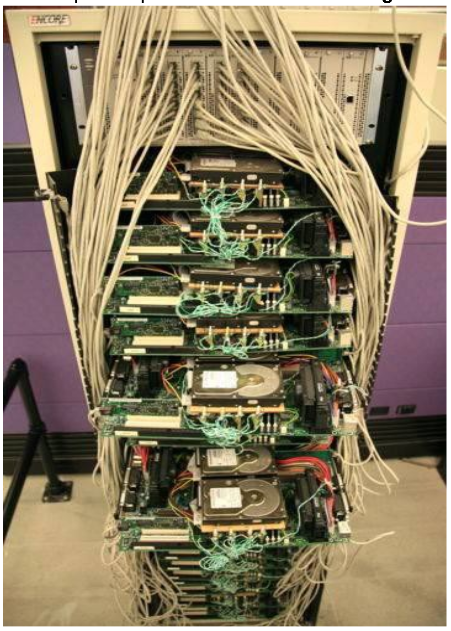
\includegraphics[width=.9\linewidth]{ArquitecturaSistemaOperativo/SO_Google.PNG}
\end{center}

En la imagen anterior podemos ver el primer servidor funcional que uso
\textbf{Google}. Como vemos, se basa en varios ordenadores instalados
conjuntamente, a los que se les retiró simplemente la caja externa para
dejar solo su contenido, a fin de aprovechar espacio en los armarios de
comunicaciones.


\section{Versiones en Windows}
\label{sec:org227f03a}
Una vez tenemos claro que tipo de sistema operativo queremos instalar, y
con qué propósito, es necesario hacer un pequeño estudio de que versión
del mismo es la que más se adecua a nuestras necesidades.

\subsubsection{Server}
\label{sec:org7e6198a}
En los sistemas Windows, si optamos por la familia de sistemas
operativos para servidores, contamos con una serie de versiones que nos
ofrecen determinadas opciones y características.

Aquí podéis ver una tabla resumen con las diferencias entre las
versiones.

\begin{center}
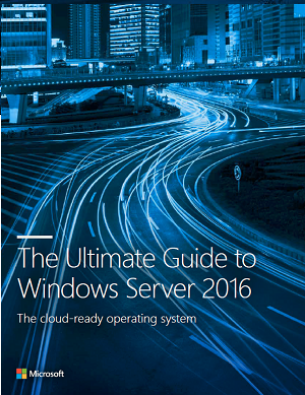
\includegraphics[width=5cm]{Versiones/WindowsServer_cover.png}
\end{center}  

\subsubsection{Windows <= 10}
\label{sec:orgf2da419}
Los sistemas Windows para escritorio han pasado por un montón de
versiones, desde Windows 3.11 a Windows 10. Estas versiones han ido
apareciendo en el tiempo y su soporte por parte de Microsoft ha ido
\emph{caducando}.

\begin{center}
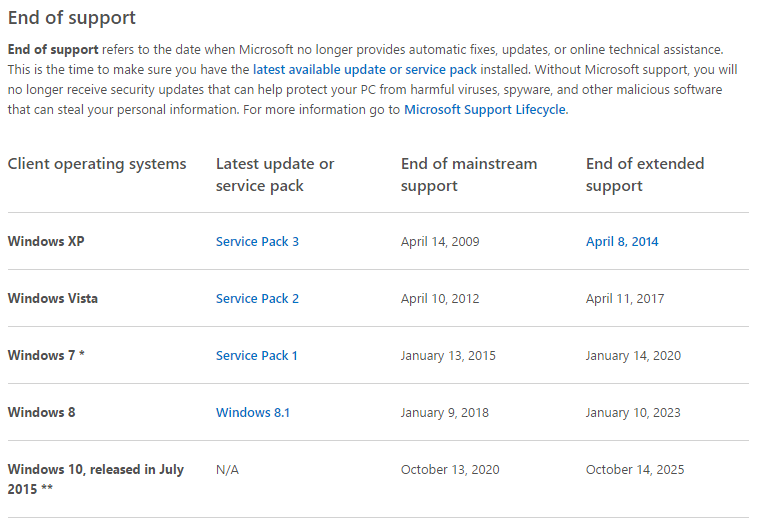
\includegraphics[width=.9\linewidth]{Versiones/fin-soporte-windows.png}
\end{center}  

\subsubsection{Actualizaciones de Windows 10}
\label{sec:org63e1d15}
Windows 10 incluye actualizaciones de manera constante, ya veremos más
adelante en el módulo porqué se realizan estos cambios, es importante
que por ahora tengamos en cuenta que es conveniente mantener nuestros
sistemas actualizados y que es una buena práctica revisar las páginas
oficiales de seguridad de los sistemas operativos que tenemos instalados
en los equipos de los que somos responsables.

\href{https://support.microsoft.com/es-es/help/4464619/windows-10-update-history}{Actualizaciones
de Windows 10}

Windows 10 ha cambiado respecto a los sistemas anteriores de Windows,
permitiendo siempre la actualización a la última versión disponible
(actualmente estamos en la de mayo de 2020). De esta manera ofrece características
de seguridad y no deben preocuparse de mantener software que no se
actualiza. Esto lo veremos más adelante en profundidad.

\begin{center}
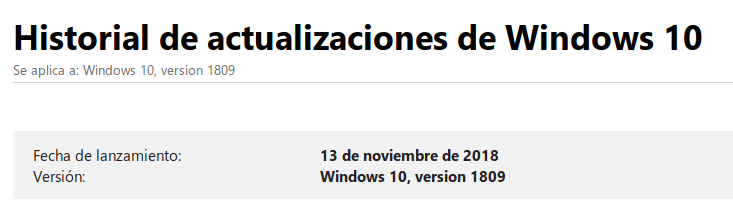
\includegraphics[width=.9\linewidth]{Versiones/windows10-1809.png}
\end{center}  

\newpage
\section{Distribuciones de GNU/LinuX}
\label{sec:orgd624b8e}
Los sistemas GNU/LinuX son muy variados, ya que multitud de comunidades
han realizado sus propias adaptaciones y selección de aplicaciones que
desean llevar \emph{por defecto}. Existen multitud de empresas que utilizan
GNU/LinuX, desde Red Hat (IBM), Canonical (Ubuntu), Microsoft, y otras
que aunque lo utilizan no ponen su marca en ella, uno de los ejemplos es
Android y Google.

El núcleo (LinuX) + Herramientas (GNU) es lo que da lugar al sistema
básico sobre el que las distribuciones y empresas trabajan.

\begin{center}
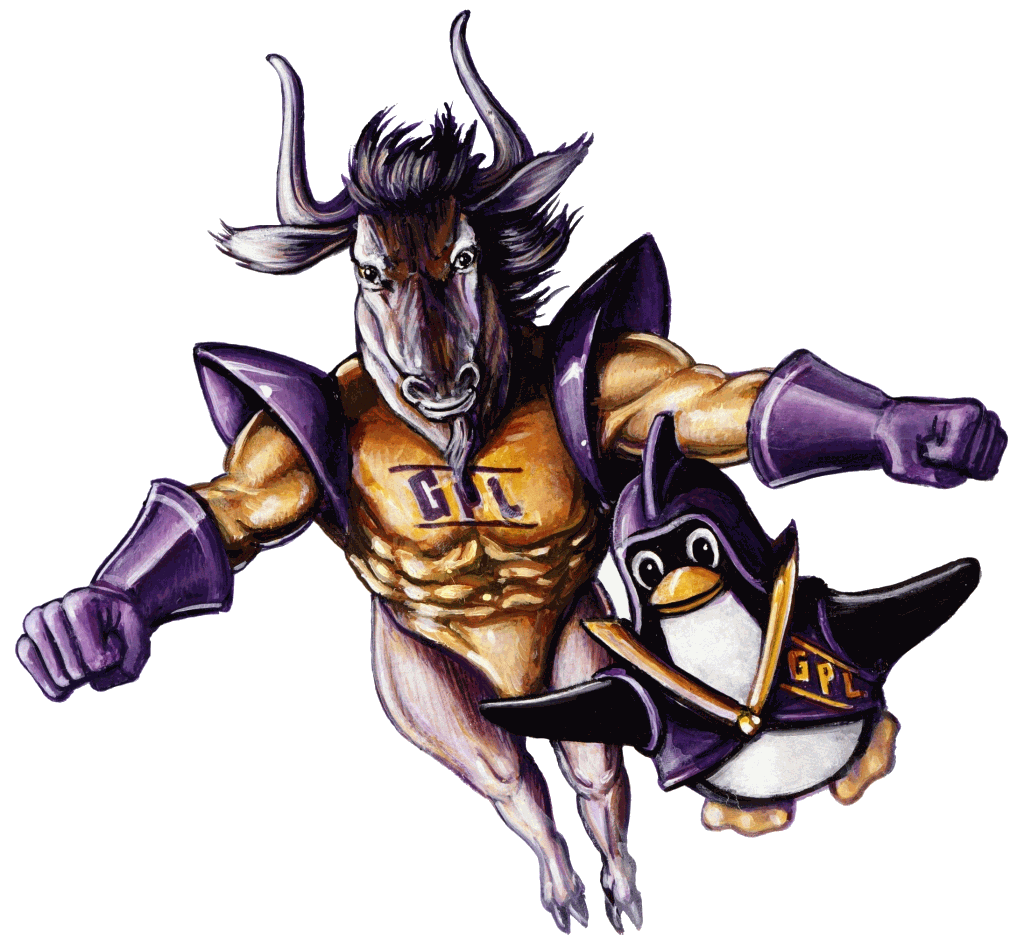
\includegraphics[width=.9\linewidth]{Versiones/Gnu-and-penguin-color.png}
\end{center}  

\newpage
\subsubsection{Un poco de historia}
\label{sec:orgcc3c775}
En la década de 1970 \texttt{UNIX} era un sistema operativo no libre o
privativo muy popular entre los reducidos usuarios académicos e
industriales de la época.

Su éxito es atribuido a :

\begin{itemize}
\item La Portabilidad.
\item Arquitectura Simple
\item Estable
\item Prácticas Liberales de Distribución de Software
\item Regulaciones \emph{anti-monopolio}, que obligaron durante un tiempo a su
propietario (\textbf{AT\&T}) a ofrecer el código gratuitamente a diversas
instituciones.
\end{itemize}

\subsubsection{Richard Stallman}
\label{sec:org7dae27c}
Mientras tanto Stallman venía de una tradición de programadores
completamente distinta en los laboratorios del MIT.

\begin{center}
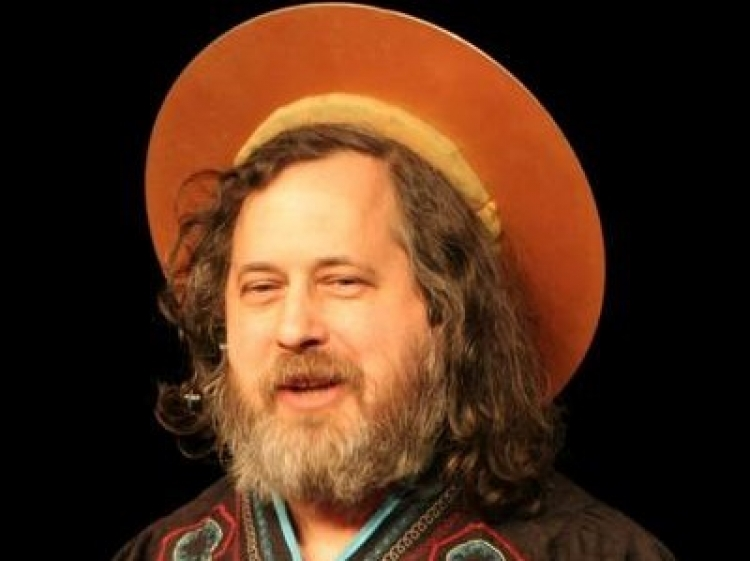
\includegraphics[width=.9\linewidth]{Versiones/stallman.jpg}
\end{center}  

Hacia principios de la década de 1980 la comunidad \emph{hacker} del MIT se
desmoronaba junto con sus sistemas.

Habiéndose acostrumbrado a modificar y compartir tales programas en
extinción; Stallman asegura que el desarrollo de un sistema operativo
libre moderno y portátil (y con éste el lanzamiento del movimiento del
software libre) fue una reacción contra lo que de otra manera le parecía
un futuro desagradable rodeado de software privativo.

Así el sistema GNU fue diseñado para ser totalmente compatible con UNIX;
aprovechando tanto el diseño modular y portable como sus usuarios.

\subsubsection{Linus Torvalds}
\label{sec:orgb85a87f}
Armado con las herramientas de GNU, en 1991 Linus Torvalds empezó a
escribir el núcleo Linux inspirado en el libro de Minix de Andrew
Tanenbaum (otro de los grandes).

\begin{center}
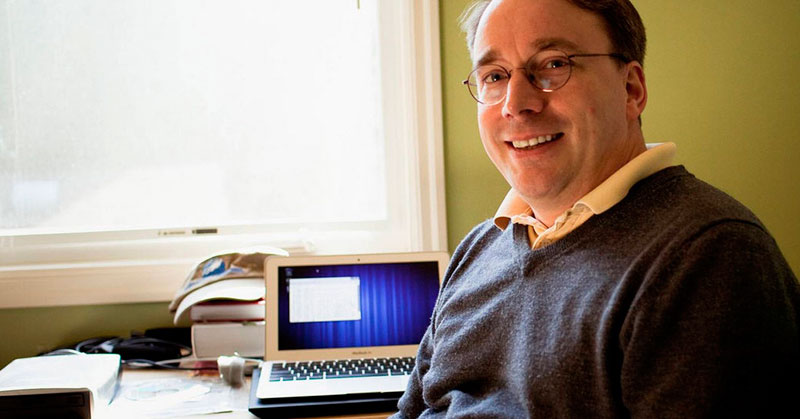
\includegraphics[width=.9\linewidth]{Versiones/Linus-Torvalds.jpg}
\end{center}  

En sus primeros anuncios públicos Torvalds le atribuía su acción a la
frustración de no poder usar Minix comercialmente, y a la ausencia de
núcleos libres tipo Unix como GNU Hurd​ o el de BSD. A pesar de sus
desacuerdos suscitados a raíz de la publicación de Linux, tanto Torvalds
como Tanenbaum pronosticaban que el superior núcleo de GNU eventualmente
dejaría obsoletos a Linux y Minix.

En 1992 Torvalds decidió cambiar la licencia no comercial de Linux a la
GPL. Rápidamente, múltiples programadores se unieron en el desarrollo,
colaborando a través de Internet y consiguiendo que paulatinamente Linux
fuera más serio, potente y compatible con UNIX.

Linux fue combinado con el resto del sistema GNU, resultando en un
sistema operativo libre y completamente funcional que sigue usándose al
día de hoy y en completa expansión.

La combinación es conocida como "GNU/Linux" o como una "distribución
Linux" y existen diversas variantes.

A lo largo del módulo, veremos muchas veces \texttt{GNU/LinuX} y \texttt{LinuX} solo,
pido disculpas a los puristas que puedan leer esta documentación. La
nomenclatura \texttt{correcta} es \textbf{GNU/LinuX}.

\subsubsection{Distribuciones y familias}
\label{sec:org2e8d5cb}
Cuando una distribución se basa en una anterior, lo que normalmente
\texttt{adopta} es la manera de empaquetar y distribuir las aplicaciones que
hace disponibles para los usuarios.

Por ejemplo, las basadas en Debian, siguen utilizando \texttt{.deb} como
paquetes de instalación, así como repositorios que disponen de esos debs
de una determinada estructura.

\begin{center}

\includegraphics[width=5cm]{Versiones/debian_ubuntu.jpg}
\end{center}  

El mundo de las distribuciones es muy complejo, y toca estar al dia de
los movimientos de las comunidades y empresas que soportan estas
distribuciones.

Aqui adjunto un enlace a las distribuciones de GNU/LinuX más famosas:

\href{https://upload.wikimedia.org/wikipedia/commons/1/1b/Linux\_Distribution\_Timeline.svg}{Distribuciones}

\subsubsection{Distribuciones Famosas}
\label{sec:org17146b1}
\begin{enumerate}
\item Debian
\label{sec:orgecc390e}
\begin{center}

\includegraphics[width=5cm]{Versiones/debian.jpeg}
\end{center}  

\href{https://www.debian.org/intro/about\#what}{Debian}

\item Ubuntu
\label{sec:org43291d4}
\begin{center}

\includegraphics[width=5cm]{Versiones/ubuntu-logo.png}
\end{center}

\href{https://www.ubuntu.com/}{Ubuntu}

\item Fedora
\label{sec:org40c1da1}
\begin{center}

\includegraphics[width=5cm]{Versiones/fedora.png}
\end{center}

\href{https://getfedora.org/es/}{Fedora}

\item RedHat
\label{sec:orgb7089eb}
\begin{center}

\includegraphics[width=5cm]{Versiones/redhat.svg.png}
\end{center}  

\href{https://www.redhat.com/es}{Red Hat}

\item OpenSuse
\label{sec:org53143bb}
\begin{center}

\includegraphics[width=5cm]{Versiones/opensuse.png}
\end{center}  

\href{https://www.opensuse.org/}{OpenSuse}

\item Archlinux
\label{sec:org00c50de}
\begin{center}

\includegraphics[width=5cm]{Versiones/archlinux.png}
\end{center}  

\href{https://www.archlinux.org/}{ArchLinux}

\item Alpine
\label{sec:org9eec190}
\begin{center}

\includegraphics[width=5cm]{Versiones/alpine.png}
\end{center}

\href{https://alpinelinux.org/}{Alpine}


\newpage
\end{enumerate}

\subsection{Tarea 02 [ CLIL ] : Manual del nano.}
\label{sec:org18cb612}

Lee atentamente el texto siguiente y contesta en \emph{castellano} a las 
preguntas que aparecen a continuación del mismo.

\begin{center}
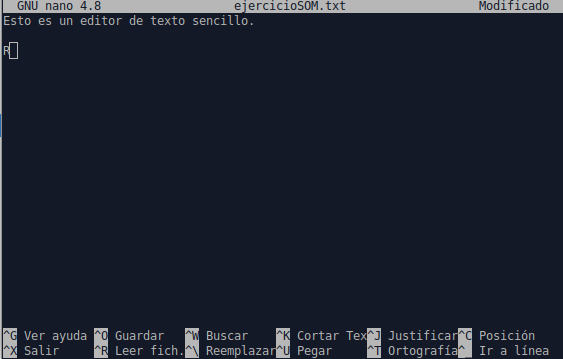
\includegraphics[width=10cm]{./imgs/nano-ejemplo.png}
\end{center}

\ldots{}

\texttt{nano is a small, free and friendly editor which aims to replace Pico,} 
\texttt{the default editor included in the non-free Pine package.} 

\texttt{Rather than just copying Pico's look and feel,}
\texttt{nano also implements some missing (or disabled by default) features in Pico,} 
\texttt{such as "search and replace" and "go to line and column number".}

\ldots{} 

\emph{From :}  \texttt{man nano}

Preguntas:

\begin{enumerate}
\item ¿Qué quiere decir la expresión: \emph{aims to replace Pico}.?
\item ¿Qué significa la palabra : \emph{default}?.
\item ¿Por qué expresión sustituirías las palabras : /look and feel/RR?
\item ¿Qué significa la expresión : \emph{missing features}?.
\item Utilizando el manual de nano:

\begin{itemize}
\item ¿Qué atajo de teclado nos permite realizar la acción de \texttt{search and replace}?
\item ¿Qué atajo de teclado nos permite realizar la acción de \texttt{go to line and column number}?
\end{itemize}
\end{enumerate}


\subsection{Tarea 03 - Ampliación [ CLIL ] : Fragmento de RMS}
\label{sec:org46edbf8}

Lee atentamente el texto siguiente y contesta en \emph{castellano} a las 
preguntas que aparecen a continuación del mismo:

\ldots{}

\emph{Other users consider proprietary manuals acceptable for the same reason so many}
\emph{people consider proprietary software acceptable: they judge in purely practical}
\emph{terms, not using freedom as a criterion. These people are entitled to their opin-}
\emph{ions, but since those opinions spring from values which do not include freedom,}
\emph{they are no guide for those of us who do value freedom.}

\ldots{}

From : \emph{Free Software needs Free Documentation} by \emph{Richard Stallman}.


\begin{enumerate}
\item ¿Qué quiere decir la expresión : \emph{entitled to their opinions}?
\item En la última frase del texto, ¿qué nos indica la expresión : \ldots{} \emph{spring from values} \ldots{}?
\item La expresión "\emph{Free as in freedom not as in free beer}" que se refiere en el mundo del Software Libre, ¿qué nos indica?.
\item ¿El autor valora la libertad?. Razona la respuesta.
\end{enumerate}

\subsection{Tarea 04 - Ampliación [ CLIL ] : Texto completo RMS}
\label{sec:org174667b}

Lee todo el artículo de Richard Stallman acerca de la documentación y formate una opinión acerca del tema.
Puedes estar deacuerdo o en desacuerdo con él, pero redacta en varias líneas tu postura. \textbf{En castellano}.
\end{document}
